% !TEX root = ../../../main.tex

\toggletrue{image}
\togglefalse{imagehover}
\chapterimage{logic_gatter_joke}
\chapterimagetitle{\uppercase{Hamlet}}
\chapterimageurl{William Shakespeare}
\toggletrue{imagehover}

\chapter{Grundgatter}
\label{chapter-grundgatter}

Logische Gatter (engl. logic gates) bilden die Grundlage aller Computerbauteile. Ein \textbf{Logikgatter} ist eine elektronische Schaltung. Es gibt \textbf{drei Grundgatter}, aus denen alle anderen Bauteile aufgebaut sind. Die Lernziele sind:\\

\newcommand{\grundgatterLernziele}{
\protect\begin{minipage}{\textwidth}
\begin{todolist}
\item Sie erklären, was wir unter einem Logikgatter verstehen.
\item Sie erklären anhand eines Beispiels das Verhalten der drei Logikgatter \texttt{UND}, \texttt{ODER} und \texttt{NICHT}.
\item Sie stellen die drei Logikgatter \texttt{UND}, \texttt{ODER} und \texttt{NICHT} grafisch dar.
\end{todolist}
\end{minipage}
}

\lernziel{\autoref{chapter-grundgatter}, \nameref{chapter-grundgatter}}{\protect\grundgatterLernziele}

\grundgatterLernziele

\section{\texttt{UND}-Gatter}

Das \texttt{UND}-Gatter (engl. \texttt{AND}-Gate\footnote{Gatter (bzw. Gate) ist die Abkürzung für Logikgatter bzw. Logic Gate.}) hat das Verhalten, dass die Glühlampe nur dann leuchtet, wenn \textbf{beide Schalter} gedrückt werden (siehe \autoref{logicly-and}).

\begin{figure}[htb]
\centering
\begin{minipage}{0.225\textwidth}
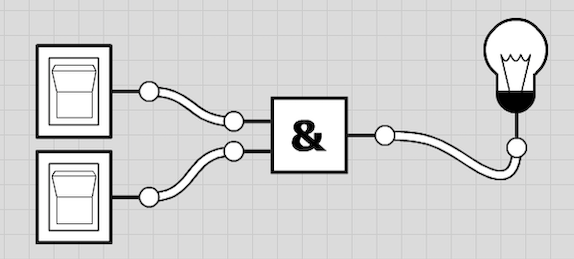
\includegraphics[width=\textwidth]{./and/and_off_off}
\end{minipage}
\begin{minipage}{0.225\textwidth}
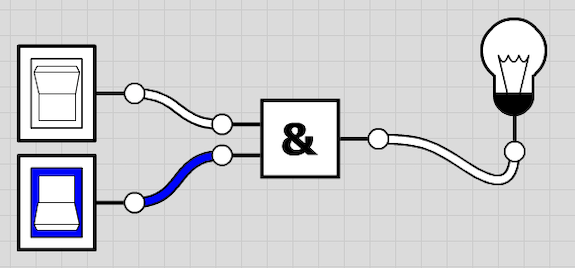
\includegraphics[width=\textwidth]{./and/and_off_on}
\end{minipage}
\begin{minipage}{0.225\textwidth}
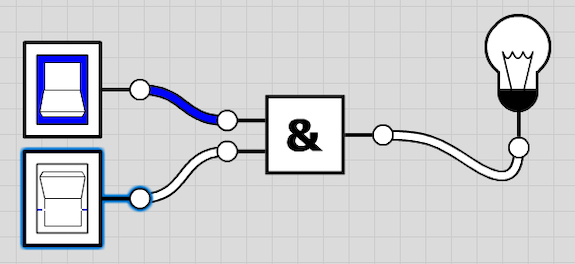
\includegraphics[width=\textwidth]{./and/and_on_off}
\end{minipage}
\begin{minipage}{0.225\textwidth}
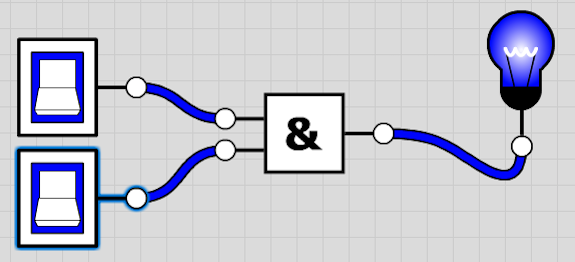
\includegraphics[width=\textwidth]{./and/and_on_on}
\end{minipage}
\caption{Es gibt vier Kombinationen, wie die Schalter betätigt werden können \cite{bowlerhat2023logicly}.}
\label{logicly-and}
\end{figure}

Wenn wir die Bauteile von Hand zeichnen, dann ist es einfacher, wenn wir die Schalter und die Glühlampen nicht zeichnen müssen. Wir nennen die Schalter als \textbf{Eingänge} und die Glühlampen \textbf{Ausgang}. Das \texttt{UND}-Gatter in \autoref{logicly-and} hat \textbf{zwei Eingänge}. Wir kürzen einen Eingang mit $E$ ab und geben jedem Eingang eine Nummer. Das Gatter hat auch \textbf{einen Ausgang}. Diesen kürzen wir mit $A_0$ ab. \autoref{circuit-and} zeigt die kompakte Darstellung, wie sie in der Digitaltechnik üblich ist.

\begin{figure}[htb]
\centering
\begin{circuitikz}
\draw (0,0) node[and port] (AND1) {}
(AND1.in 1) node[anchor=east] {$E_0$} 
(AND1.in 2) node[anchor=east] {$E_1$}
(AND1.out) node[anchor=west] {$A_0$};
\end{circuitikz}
\caption{Das \texttt{UND}-Gatter besteht aus einem Rechteck mit einem \protect\say{Kaufmanns-Und} (engl. ampersand) darin. Die Eingänge werden immer auf der linken, die Ausgänge auf der rechten Seite des Bauteils gezeichnet.}
\label{circuit-and}
\end{figure}

Die Funktionsweise des \texttt{UND}-Gatters lässt sich auch gut anhand eines Schaltplans veranschaulichen (siehe \autoref{circuit-and-schaltplan}). Die Glühlampe leuchtet nur, wenn der Schalter $E_0$ und der Schalter $E_1$ gedrückt sind. Die Schalter sind sogenannte Schliesser. Wenn sie gedrückt sind, ist der Stromkreis geschlossen. Dann kann der Strom von der Batterie in Pfeilrichtung zur Glühlampe fliessen.

\begin{figure}[htb]
\centering
\begin{circuitikz}
\draw (0,0) to (1,0) to[cute open switch, label=$E_0$] (2.5,0) to (3.5,0) to[cute open switch, label=$E_1$] (5.5,0)
to (5.5, -1) to[lamp, label=$A_0$] (2.5, -1) to[battery1=\SI{5}{V}] (0,-1) to (0,0);
\end{circuitikz}
\caption{Zwei Schalter ($E_0$ und $E_1$), eine Batterie (Spannungsquelle) und eine Lampe ($A_0$).}
\label{circuit-and-schaltplan}
\end{figure}

\section{\texttt{ODER}-Gatter}

Das \texttt{ODER}-Gatter (engl. \texttt{OR}-Gate) hat das Verhalten, dass die Glühlampe nur dann leuchtet, wenn \textbf{mindestens} ein Schalter gedrückt wird (siehe \autoref{logicly-or}).

\begin{figure}[htb]
\centering
\begin{minipage}{0.225\textwidth}
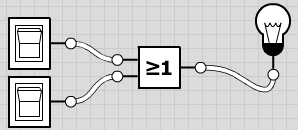
\includegraphics[width=\textwidth]{./or/or_off_off}
\end{minipage}
\begin{minipage}{0.225\textwidth}
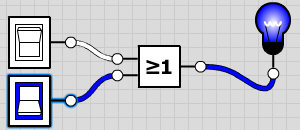
\includegraphics[width=\textwidth]{./or/or_off_on}
\end{minipage}
\begin{minipage}{0.225\textwidth}
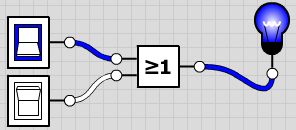
\includegraphics[width=\textwidth]{./or/or_on_off}
\end{minipage}
\begin{minipage}{0.225\textwidth}
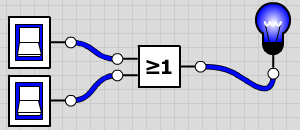
\includegraphics[width=\textwidth]{./or/or_on_on}
\end{minipage}
\caption{Es dürfen auch beide Schalter gedrückt werden.}
\label{logicly-or}
\end{figure}

Wir zeichnen das \texttt{ODER}-Gatter (siehe \autoref{circuit-or}) mit zwei Eingängen und einem Ausgang.

\begin{figure}[htb]
\centering
\begin{circuitikz}
\draw (0,0) node[or port] (OR1) {}
(OR1.in 1) node[anchor=east] {$E_0$} 
(OR1.in 2) node[anchor=east] {$E_1$}
(OR1.out) node[anchor=west] {$A_0$};
\end{circuitikz}
\caption{\texttt{ODER}-Gatter: Rechteck mit einem Grösser-Gleich-Zeichen ($\geq$) und einer \num{1} darin.}
\label{circuit-or}
\end{figure}

Die Funktionsweise des \texttt{ODER}-Gatters ist in \autoref{circuit-or-schaltplan} als elektrischer Schaltplan dargestellt.

\begin{figure}[H]
\centering
\begin{circuitikz}
\draw (0,0) to (1,0) to (1, 0.5) to (2, 0.5) to[cute open switch, label=$E_0$] (3.5, 0.5) to (4, 0.5) to (4, 0);
\draw (0,0) to (1,0) to (1, -0.75) to (2, -0.75) to[cute open switch, label=$E_1$] (3.5, -0.75) to (4, -0.75) to (4, 0);
\draw (4,0) to (5.5, 0) to (5.5, -1.5) to[lamp, label=$A_0$] (2.5, -1.5) to[battery1=\SI{5}{V}] (0,-1.5) to (0,0);
\end{circuitikz}
\caption{Mindestens ein Schalter muss gedrückt werden, damit die Glühlampe leuchtet.}
\label{circuit-or-schaltplan}
\end{figure}

\section{\texttt{NICHT}-Gatter}

Das \texttt{NICHT}-Gatter (engl. \texttt{NOT}-Gate) hat das Verhalten, dass die Glühlampe nur dann leuchtet, wenn der Schalter \textbf{nicht} gedrückt ist (siehe \autoref{logicly-not}).

\begin{figure}[H]
\centering
\begin{minipage}{0.25\textwidth}
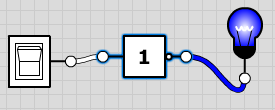
\includegraphics[width=\textwidth]{./not/not_off}
\end{minipage}
\begin{minipage}{0.25\textwidth}
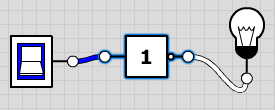
\includegraphics[width=\textwidth]{./not/not_on}
\end{minipage}
\caption{Das \texttt{NICHT}-Gatter hat nur einen Eingang.}
\label{logicly-not}
\end{figure}

Das \texttt{NICHT}-Gatter \say{dreht} den Strom sozusagen um. Deshalb nennen wir dieses Gatter \textbf{Inverter}\footnote{Invertieren bedeutet umkehren beziehungsweise umdrehen.}. Wir zeichnen das Gatter mit \textbf{einem} Eingang und \textbf{einem} Ausgang (siehe \autoref{circuit-not}).

\begin{figure}[ht]
\centering
\begin{minipage}{0.45\textwidth}
\centering
\begin{circuitikz}
\draw (0,0) node[european not port] (NOT1) {}
(NOT1.in) node[anchor=east] {$E_0$} 
(NOT1.out) node[anchor=west] {$A_0$};
\end{circuitikz}
\caption{\texttt{NICHT}-Gatter: ausserhalb des Rechtecks ist ein Kreis eingezeichnet.}
\label{circuit-not}
\end{minipage}
\hfill
\begin{minipage}{0.45\textwidth}
\centering
\begin{circuitikz}
\draw (0,0) node[buffer port] (BUFFER1) {}
(BUFFER1.in 1) node[anchor=east] {$E_0$} 
(BUFFER1.out) node[anchor=west] {$A_0$};
\end{circuitikz}
\caption{\texttt{BUFFER}-Gatter: besteht aus einem Rechteck mit einer \num{1} darin.}
\label{circuit-buffer}
\end{minipage}
\end{figure}

Wir können uns die Darstellung des \texttt{NICHT}-Gatters besser vorstellen, wenn wir zunächst das \texttt{BUFFER}-Gatter betrachten. Das \texttt{BUFFER}-Gatter leitet den Strom einfach unverändert weiter. Der Kreis beim \texttt{NICHT}-Gatter symbolisiert das \protect\say{Umdrehen} des Stromes. Die Funktionsweise des \texttt{NICHT}-Gatters ist in \autoref{circuit-not-schaltplan} als elektrischen Schaltplan dargestellt. Der Schalter $E_0$ ist ein so genannter Öffner. Wird der Öffner betätigt, ist der Stromkreis unterbrochen. Nur wenn der Öffner \textbf{nicht} gedrückt ist, kann der Strom in Pfeilrichtung fliessen und die Glühlampe leuchtet.

\begin{figure}[htb]
\centering
\begin{circuitikz}
\draw (0,0) to (1,0) to[normal closed switch, label=$E_0$] (2.5,0) to (3.5,0) to (5.5,0)
to (5.5, -1) to[lamp, label=$A_0$] (2.5, -1) to[battery1=\SI{5}{V}] (0,-1) to (0,0);
\end{circuitikz}
\caption{Wir drücken von \protect\say{unten} gegen den Öffner und dann wird der Strom unterbrochen.}
\label{circuit-not-schaltplan}
\end{figure}

\section{Übungen}

\begin{exercise}\label{uebung-autobeleuchtung}
\autoref{figure-logikgatter-uebung-oder} zeigt zwei Fahrzeugtüren. Solange eine Autotür geöffnet ist, soll das Licht im Auto eingeschaltet sein. Tragen Sie das entsprechende Logikgatter für diese Situation ein.

\begin{figure}[htb]
\centering
\begin{minipage}{0.275\textwidth}
\centering
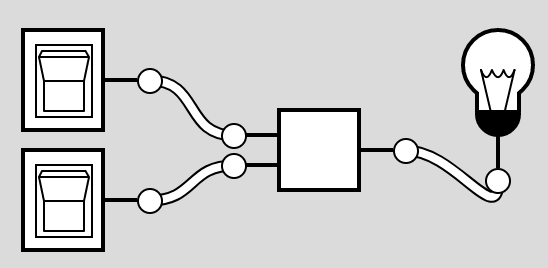
\includegraphics[height=2cm]{logikgatter_uebung_oder}
\caption{Übung \ref{uebung-autobeleuchtung}}
\label{figure-logikgatter-uebung-oder}
\end{minipage}
\hfill
\begin{minipage}{0.275\textwidth}
\centering
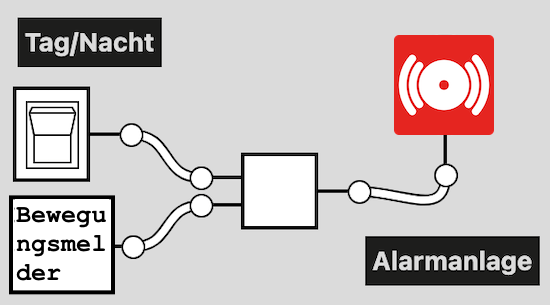
\includegraphics[height=2cm]{logikgatter_uebung_und}
\caption{Übung \ref{uebung-alarm}}
\label{figure-logikgatter-uebung-und}
\centering
\end{minipage}
\hfill
\begin{minipage}{0.35\textwidth}
\centering
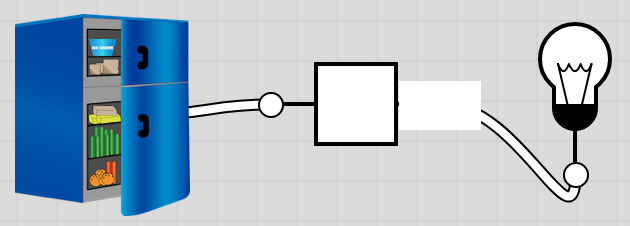
\includegraphics[height=2cm]{logikgatter_uebung_nicht}
\caption{Übung \ref{uebung-kuehlschrank}}
\label{figure-logikgatter-uebung-nicht}
\centering
\end{minipage}
\end{figure}
\end{exercise}

\begin{exercise}\label{uebung-alarm}
In einem Museum ist ein Bewegungsmelder (siehe \autoref{figure-logikgatter-uebung-und}) installiert. Der Bewegungsmelder soll nur nachts einen Alarm auslösen. Dazu schaltet der Nachtwächter das Überwachungssystem mit einem Schalter \say{scharf}. Tragen Sie das entsprechende Logikgatter für diese Situation ein.
\end{exercise}

\begin{exercise}\label{uebung-kuehlschrank}
Das Licht in einem Kühlschrank (siehe \autoref{figure-logikgatter-uebung-nicht}) leuchtet nur, wenn die Tür geöffnet ist. Dazu betätigt die Tür einen Schalter, wenn sie geschlossen ist. Tragen Sie das entsprechende Logikgatter für diese Situation ein.
\end{exercise}
